
\chapter{Literature Review}

\section{Abnormal Heart Sound Detection}

% Cardiovascular diseases (CVDs) continue to be the top cause of death worldwide, making early diagnosis a critical step in saving lives and improving quality of care. While advanced tools like echocardiograms and ECGs are commonly available in high-income countries, many low- and middle-income regions lack the resources to access these technologies. In such contexts, heart auscultation—the practice of listening to heart sounds using a stethoscope—offers a practical, non-invasive, and affordable way to screen for abnormalities like murmurs, valve disorders, and arrhythmias. However, the reliability of auscultation depends greatly on the experience and skill of the clinician, leading to inconsistencies and potential diagnostic errors.

% To address this, the field has seen significant progress with computer-aided auscultation (CAA) systems. These tools pair digital stethoscopes with signal processing and machine learning techniques to automate and standardize heart sound analysis \cite{swarup2018digital}. They extract key features from phonocardiogram (PCG) recordings—such as energy, entropy, time-frequency patterns, and wavelet coefficients—to identify components like the first (S1) and second (S2) heart sounds, as well as murmurs and abnormal extra sounds \cite{li2020review, qian2019deep}. Traditional machine learning models, including support vector machines (SVMs), decision trees, and random forests, have shown promising results, particularly when trained on curated datasets.

% With the emergence of deep learning, more sophisticated models like convolutional neural networks (CNNs) and recurrent neural networks (RNNs) have been used to capture intricate patterns directly from raw or preprocessed PCG signals \cite{winther2021advanced, clifford2016classification}. Many recent approaches combine both 1D audio signals and 2D visual representations—such as spectrograms—to leverage complementary information and boost classification accuracy. Public datasets like the PhysioNet/CinC 2016 Challenge have played a key role by offering a wide range of expert-labeled PCG recordings for training and evaluation \cite{clifford2016classification, liu2016openaccess}.

Cardiovascular diseases (CVDs) remain the leading cause of mortality globally, emphasizing the need for early and accurate diagnosis to improve patient outcomes and quality of care. While diagnostic tools such as echocardiograms and electrocardiograms (ECGs) are standard in high-income countries, many low- and middle-income regions face significant challenges in accessing these technologies. In such settings, heart auscultation—the practice of listening to heart sounds using a stethoscope—serves as a practical, non-invasive, and affordable screening method for detecting abnormalities like murmurs, valve disorders, and arrhythmias. However, the effectiveness of auscultation heavily relies on the clinician's expertise, which can result in inconsistent interpretations and diagnostic errors.

To overcome these limitations, significant progress has been made in computer-aided auscultation (CAA) systems. These systems combine digital stethoscopes with advanced signal processing and machine learning algorithms to enable automated and standardized analysis of heart sounds \cite{swarup2018digital}. CAA systems extract relevant features from phonocardiogram (PCG) signals—such as energy, entropy, time-frequency characteristics, and wavelet transforms—to detect key components like the first (S1) and second (S2) heart sounds, murmurs, and abnormal extra sounds \cite{li2020review, qian2019deep}. Traditional machine learning methods, including support vector machines (SVMs), decision trees, and random forests, have demonstrated strong performance when applied to well-annotated datasets.

The advent of deep learning has further enhanced these capabilities, with models such as convolutional neural networks (CNNs) and recurrent neural networks (RNNs) being utilized to learn complex patterns from raw or preprocessed PCG recordings \cite{winther2021advanced, clifford2016classification}. Modern approaches often integrate both 1D audio waveforms and 2D visual features—like spectrograms—to capture complementary information and improve classification accuracy. The availability of publicly accessible datasets, such as those from the PhysioNet/CinC 2016 Challenge, has greatly facilitated the development and benchmarking of these systems by providing a wide array of expert-labeled heart sound recordings \cite{clifford2016classification, liu2016openaccess}.


\begin{figure}[htbp]
    \centering
    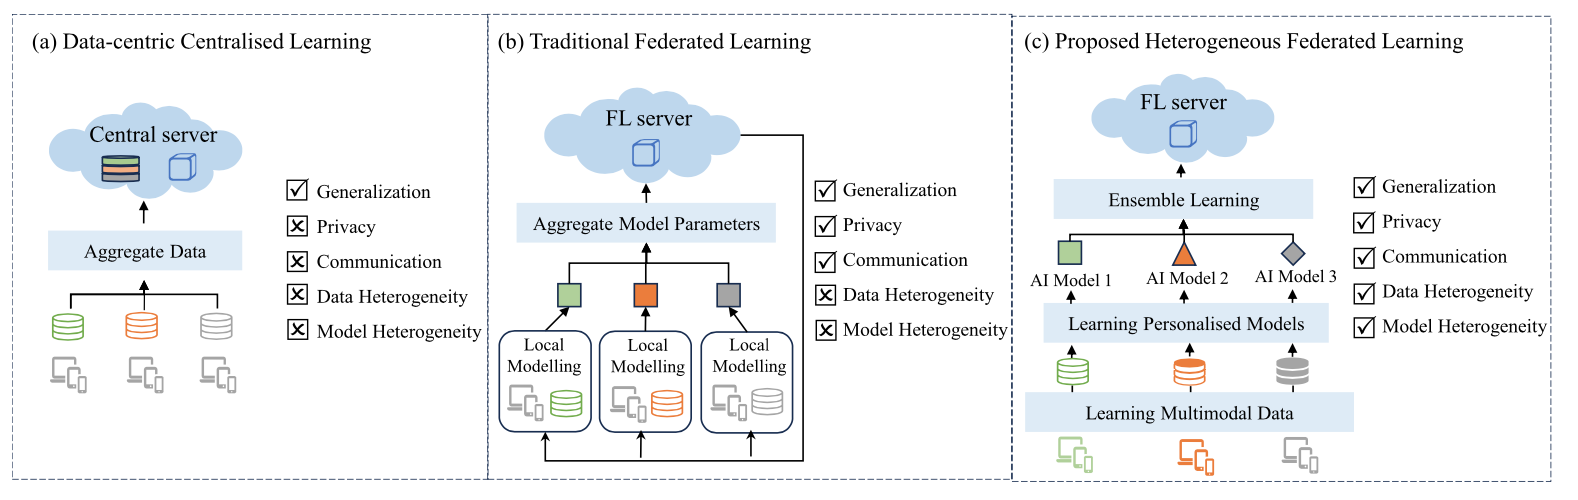
\includegraphics [width=0.9\textwidth]{./Figures/fig.png}
    \caption{Research background. (a) Data-centric centralised learning, which pools data together to train a central ML model. (b) In traditional FL, the global model is trained under the coordination of the central server while data resides in different data silos. (c) The proposed heterogeneous FL, which addresses the limitations of FL through ensemble personalised models learning. 
}
    \label{fig:enter-label}
\end{figure}


Despite major strides in heart sound analysis, several challenges remain. One persistent issue is the variability between patients, which can affect how heart sounds are interpreted. Recordings often contain background noise or artifacts, and some critical heart conditions—like rare anomalies—are underrepresented in datasets, making it harder for models to learn from them. For AI systems to be trusted and adopted in clinical settings, they also need to generalize well across populations, be interpretable by healthcare professionals, and run efficiently on edge devices such as digital stethoscopes or wearables.

To tackle these hurdles, researchers are turning to methods like domain adaptation to help models adapt across different patient groups and clinical conditions. Explainable AI (XAI) techniques are being developed to make model decisions more transparent, helping clinicians understand why a certain prediction was made. Meanwhile, privacy-preserving approaches like federated learning are gaining traction, enabling collaborative model training without sharing sensitive patient data. Together, these innovations are paving the way toward a scalable and equitable future for AI-powered heart sound diagnostics—one that could benefit patients around the world regardless of where they live.

\section{AI and IoHT in Remote Healthcare}

The Internet of Health Things (IoHT) brings together wearable devices, mobile health applications, and smart sensors to enable continuous patient monitoring and real-time data collection. This integrated ecosystem allows healthcare providers to remotely track key physiological signals such as heart rate, respiration, and body temperature—an especially valuable tool for managing chronic conditions and supporting elderly populations \cite{alshamrani2022iot, qian2021artificial}.

Artificial intelligence (AI) takes this a step further by analyzing the large volumes of multimodal data generated by these devices. With AI, systems can detect early warning signs, issue timely alerts, and offer tailored health recommendations—all while reducing the workload on clinicians and giving patients more control over their care \cite{qian2021can}.

However, traditional AI systems typically rely on centralized data collection, where patient information is uploaded to remote servers for model training. While effective, this approach poses significant privacy and security risks. Healthcare data is not only sensitive but also highly regulated, and centralization increases the chance of breaches and biases—especially when the training data doesn’t reflect diverse populations \cite{xu2021federated}.

To overcome these limitations, federated learning has emerged as a powerful alternative. Rather than sharing raw data, federated learning allows models to be trained locally on each device or institution’s data and then aggregated into a shared global model. This preserves privacy, reduces data exposure, and fosters secure collaboration across different healthcare stakeholders—all while maintaining the performance benefits of modern AI.


\section{Federated Learning in Healthcare}
Federated learning (FL) offers a privacy-conscious way for healthcare institutions to collaboratively train AI models without sharing sensitive patient data~\cite{mcmahan2017communication}. Instead of moving data, each institution trains models locally and only shares model updates with a central server. Using algorithms like FedAvg, these updates are combined to build a stronger global model. As shown in Figure~\ref{fig:fl_workflow}, this process supports local training, centralized aggregation, and privacy by design. FL is already proving effective in medical use cases like disease prediction~\cite{xu2021federated}, mortality risk estimation~\cite{huang2019patient}, and secure electronic health record (EHR) sharing~\cite{brisimi2018federated, tramel2019federated}.

\begin{figure}[ht]
    \centering
    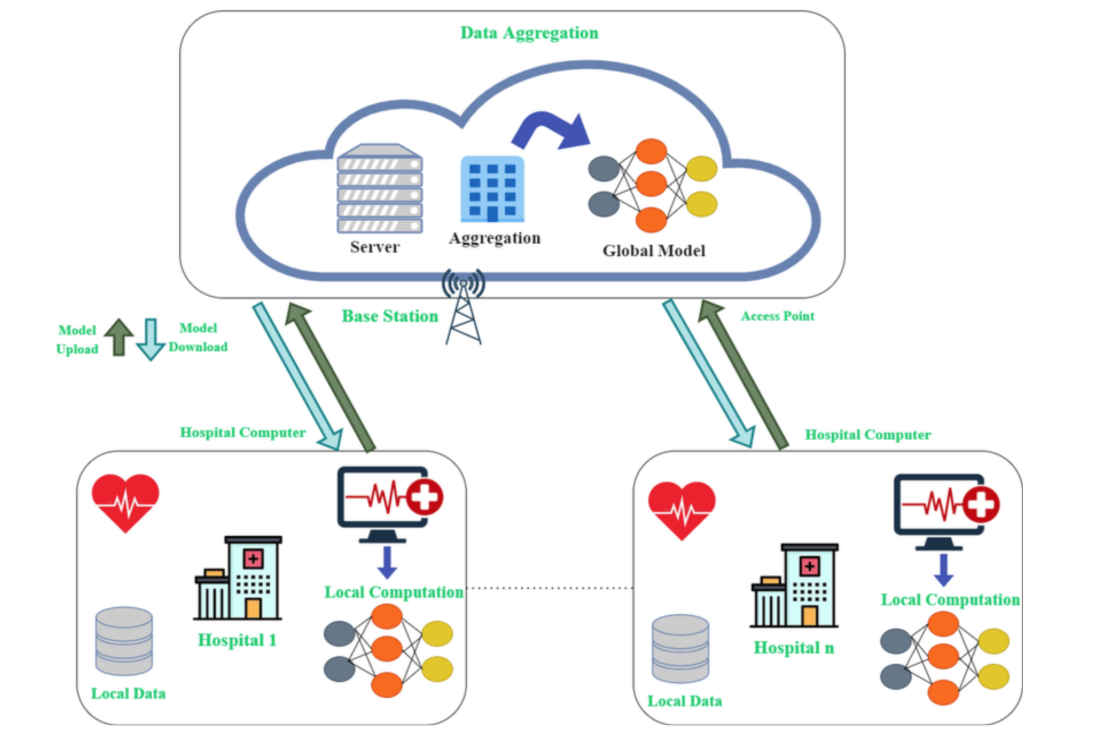
\includegraphics[width=0.9\textwidth]{./Figures/fig2.png}
    \caption{Federated learning workflow with local model training, secure aggregation, and global model distribution.}
    \label{fig:fl_workflow}
\end{figure}

Despite its promise, real-world FL systems face three major challenges, as illustrated in Figure~\ref{fig:fl_workflow}: (1) non-identical data distributions (non-IID) across institutions~\cite{nguyen2022federated}, (2) differences in local model architectures~\cite{yoo2021personalized}, and (3) incomplete class labels within client datasets~\cite{zhang2022federated}. While earlier studies~\cite{qiu2022binary, qiu2024multiclass} have shown FL’s potential for heart sound classification, they often assumed ideal scenarios—uniform models and fully aligned label spaces. For FL to succeed in clinical settings, its architecture must adapt to these real-world constraints.

\section{Personalization and Heterogeneity in FL}
To better reflect the diversity across clients in federated learning, researchers have explored several personalization strategies. These include clustered FL~\cite{yoo2021personalized}, multi-branch architectures~\cite{mori2023multi}, and client-specific training techniques  \cite{tan2023towards} \cite{huang2022learn}. Ensemble and semi-supervised approaches have also shown promise in managing non-IID settings, as seen in studies like~\cite{itahara2023distillation, shaik2022fedstack}. For instance, FedStack~\cite{shaik2022fedstack} used a stacking ensemble for personalized activity monitoring, while Liu et al.~\cite{xu2023federated} tackled inconsistent label distributions in multi-organ segmentation using federated ensembles. Collectively, these efforts highlight the potential of ensemble learning—especially model stacking—as a practical solution to heterogeneity and label misalignment in FL.

\section{Ensemble Learning and Model Stacking}
Ensemble learning techniques like bagging, boosting, and stacking are well-known for enhancing model generalization and robustness~\cite{buhlmann2012ensemble, ribeiro2020ensemble}. Among these, stacking stands out for its ability to combine diverse model architectures, making it particularly valuable in settings like network intrusion detection\cite{zhang2021multi,rajagopal2020stacking} and time-series forecasting~\cite{ribeiro2020ensemble}. In federated learning scenarios, stacking is especially effective because client models often differ in structure due to varying computational capacities or domain-specific needs~\cite{lin2020ensemble}. By training a meta-model on the predictions from these heterogeneous clients, stacking offers a practical way to integrate their outputs—an approach particularly beneficial for complex tasks like multi-class heart sound classification, where clients may have incomplete label sets~\cite{liu2024cybersecurity}.

\section{Summary and Gaps}
While previous research has applied federated learning to medical diagnostics and explored ensemble strategies for model fusion, few have tackled the combined challenges of label misalignment, client model heterogeneity, and multimodal auscultation data. Our proposed framework, \textbf{MStacking}, addresses this gap by using a stacking ensemble approach within a federated learning setup. This allows integration of insights from clients with varying model types and incomplete label spaces—conditions common in real-world healthcare. By doing so, MStacking offers a practical and scalable path toward deploying AI-assisted auscultation across diverse, decentralized medical institutions.

% \end{document}